\documentclass{article}

\usepackage{xspace}
\usepackage{xcolor}
\usepackage{amsmath}
\usepackage{amssymb}
\usepackage{amsthm}
\usepackage{amsmath}
\usepackage{graphicx}

\newtheorem{conjecture}{Conjecture}[section]
\newtheorem{corollary}{Corollary}
\newtheorem{definition}{Definition}[section]
\newtheorem{example}{Example}

\newcommand{\LTLglobally}{\Box}
\newcommand{\LTLeventually}{\Diamond}
\newcommand{\LTLnext}{\bigcirc}
\newcommand{\Name}{\textit{FormA}\xspace}
\newcommand{\cbmc}{\texttt{CBMC}}

\title{COMS 6863 Final Project Status Report: \Name{}}
\author{
    Max Levatich$^*$ \& Wonhyuk (Harry) Choi
    \footnote{Both authors contributed equally to the project.}
}
\date{\today}

\begin{document}
\maketitle

\section{Introduction}

    Our aim is to design, program, and verify via model-checking a lightweight
	video game called \Name, \emph{Formal verified Asteroids}.
	\Name is based loosely on the classic arcade
    game \textit{Asteroids} \cite{asteroids}; the player controls a small
    spaceship, viewed from a top-down perspective, and must avoid or shoot down
    incoming asteroids from all directions. The player receives points based on
    how many asteroids they destroy and how long they survive.

    \Name{} will be implemented in C, with the help of the low-level rendering
    library SDL. We will use CBMC \cite{clarke2004tool} to model-check
    certain properties of the game as we develop it, including collision
    detection, collision resolution, and input correspondence. We will submit:

    \begin{enumerate}
        \item{The game's code and assets}
        \item{Build instructions, including how to invoke CBMC}
        \item{A correctness specification of the properties checked}
        \item{A final project report detailing our process}
    \end{enumerate}

\section{Game Overview}

    \subsection{Implementation}

        \Name{} is written in C (C11 standard) and depends on Simple DirectMedia
        Layer 2.0 (SDL). SDL is a development library written in C which
        provides a simple low-level interface to the keyboard, audio, and
        graphics hardware necessary to program a video game. We will use CBMC
        to model-check the game (see Section 4).

        We will use the traditional game programming technique of a \textit{game
        loop} located in the main file, where each iteration of the loop
        represents one \textit{frame}, in which we read user input, update the
        game state, and render the game state to the screen. Modules and
        functions will be designed specifically to provide a minimal interface
        to the model-checked portions of our code. We aim to have verified
        modules which encapsulate specific features of the game (e.g. collision
        detection, keyboard input).

    \subsection{Gameplay}

        In \Name{}, the player will use the arrow keys on the keyboard to
        control a ``spaceship''. The up arrow applies a force to the ship in the
        direction that it is facing, while the left and right arrows turn the
        ship in place. This allows the player to navigate a 2D plane which wraps
        around. Asteroids will spawn randomly outside of the boundaries of the
        space with fixed velocities and the player must avoid them or shoot them
        using the spacebar, which will fire a bullet in the direction the ship
        is facing. Staying alive and shooting down asteroids increases the
        player's score. Contact with an asteroid results in a game-over.

        We are entertaining extensions to this core game which provide more
        interesting properties for us to model check, including:

        \begin{enumerate}
            \item{Non-game-ending collisions with ``bouncy'' objects. This allows
                  us to model-check properties like conservation of momentum
                  (subject to energy dissipation).}
            \item{Obstacle courses constructed out of ``planetary'' objects which
                  induce a gravitational field on the ship and asteroids. This
                  allows us to model check the proper application of the force
                  of gravity.}
			\item{``Lives'' and an ``invincibility'' mode after losing a life}
        \end{enumerate}

    \subsection{Algorithms}

        Many of the game's central mechanics revolve around collision detection
        and resolution.

        For collision detection, we will use an Axis-Aligned Bounding Box (AABB)
        algorithm with fine-grained boxes. To enable fine-grained boxes, we may
        also explore classical collision detection optimizations, which prune
        the $n^2$ space of all potential collisions (one for each pair of
        objects) into a set of \textit{candidate} collisions for objects which
        are efficiently determined to be reasonably close
        \cite{moore1988collision, palmer1995collision}. Should we implement any
        optimizations, we will aim to use model checking to show that the
        optimizations are correct; that is, they do not prune any collisions
        which should have happened on a particular frame.

\section{Correctness Specification}

    Our specification will change and grow as we develop the game and discover
    what kinds of properties we can effectively check. Here are some initial CTL
    formulas we plan to check.

    \subsection{Collision Handling}

        $AG(\forall obj. obj \neq ship \implies \lnot touching(obj,ship))$

    \subsection{Input Correspondance}

        $AG(keydown(UP) \implies ship.fx = -sin(ship.theta) * ACCEL\_NORM
                        \land ship.fy = cos(ship.theta) * ACCEL\_NORM)$

        $AG(keydown(LEFT) \land \lnot keydown(RIGHT) \implies ship.omega = ANGULAR\_VEL)$

        $AG(keydown(RIGHT) \land \lnot keydown(LEFT) \implies ship.omega = -ANGULAR\_VEL)$

        $AG(keydown(LEFT) \land keydown(RIGHT) \implies ship.omega = 0)$
	
	\subsection{Asteroid Leaves Screen}
	
		\begin{align*}
			AG((asteroid.x < 0 \lor end < asteroid.x) \land 
			(asteroid.y < 0 \lor end < asteroid.y))
		\end{align*}
    
    \subsection{Asteroids Always Exist}
    \[AG(asteroids != NULL)\]

\section{Verification Approach}

    To verify our correctness specification (Section 3), we will use the C
    Bounded Model Checker (CBMC). CBMC is capable of statically checking the
    validity of assertions in a C program by unrolling paths through the
    program.

    We plan to express the propositional logic formulas in our correctness
    specification as assertions, preconditions, and postconditions, such that
    CBMC can check them. These assertions will be invoked on every iteration of
    the \textit{game loop}, such that from a zoomed-out perspective where each
    frame of the game is a state transition, they can be viewed as AG() CTL
    formulas.

	We plan to integrate CBMC as a developmental procedure, just like regression testing might be used in a software development cycle.
	Creating the assertions themselves will help with the design process, and model checking will show that we have the correct implementation with respect to the specification.

\subsection{Comparison with \texttt{clang-tidy}}
We also employed the tool \texttt{clang-tidy} to catch possible bugs through static analysis.
Most notably, it was able to show a null pointer dereference that we had in our code (Figure~\ref{fig:clang-tidy})
\begin{figure}[!h]
    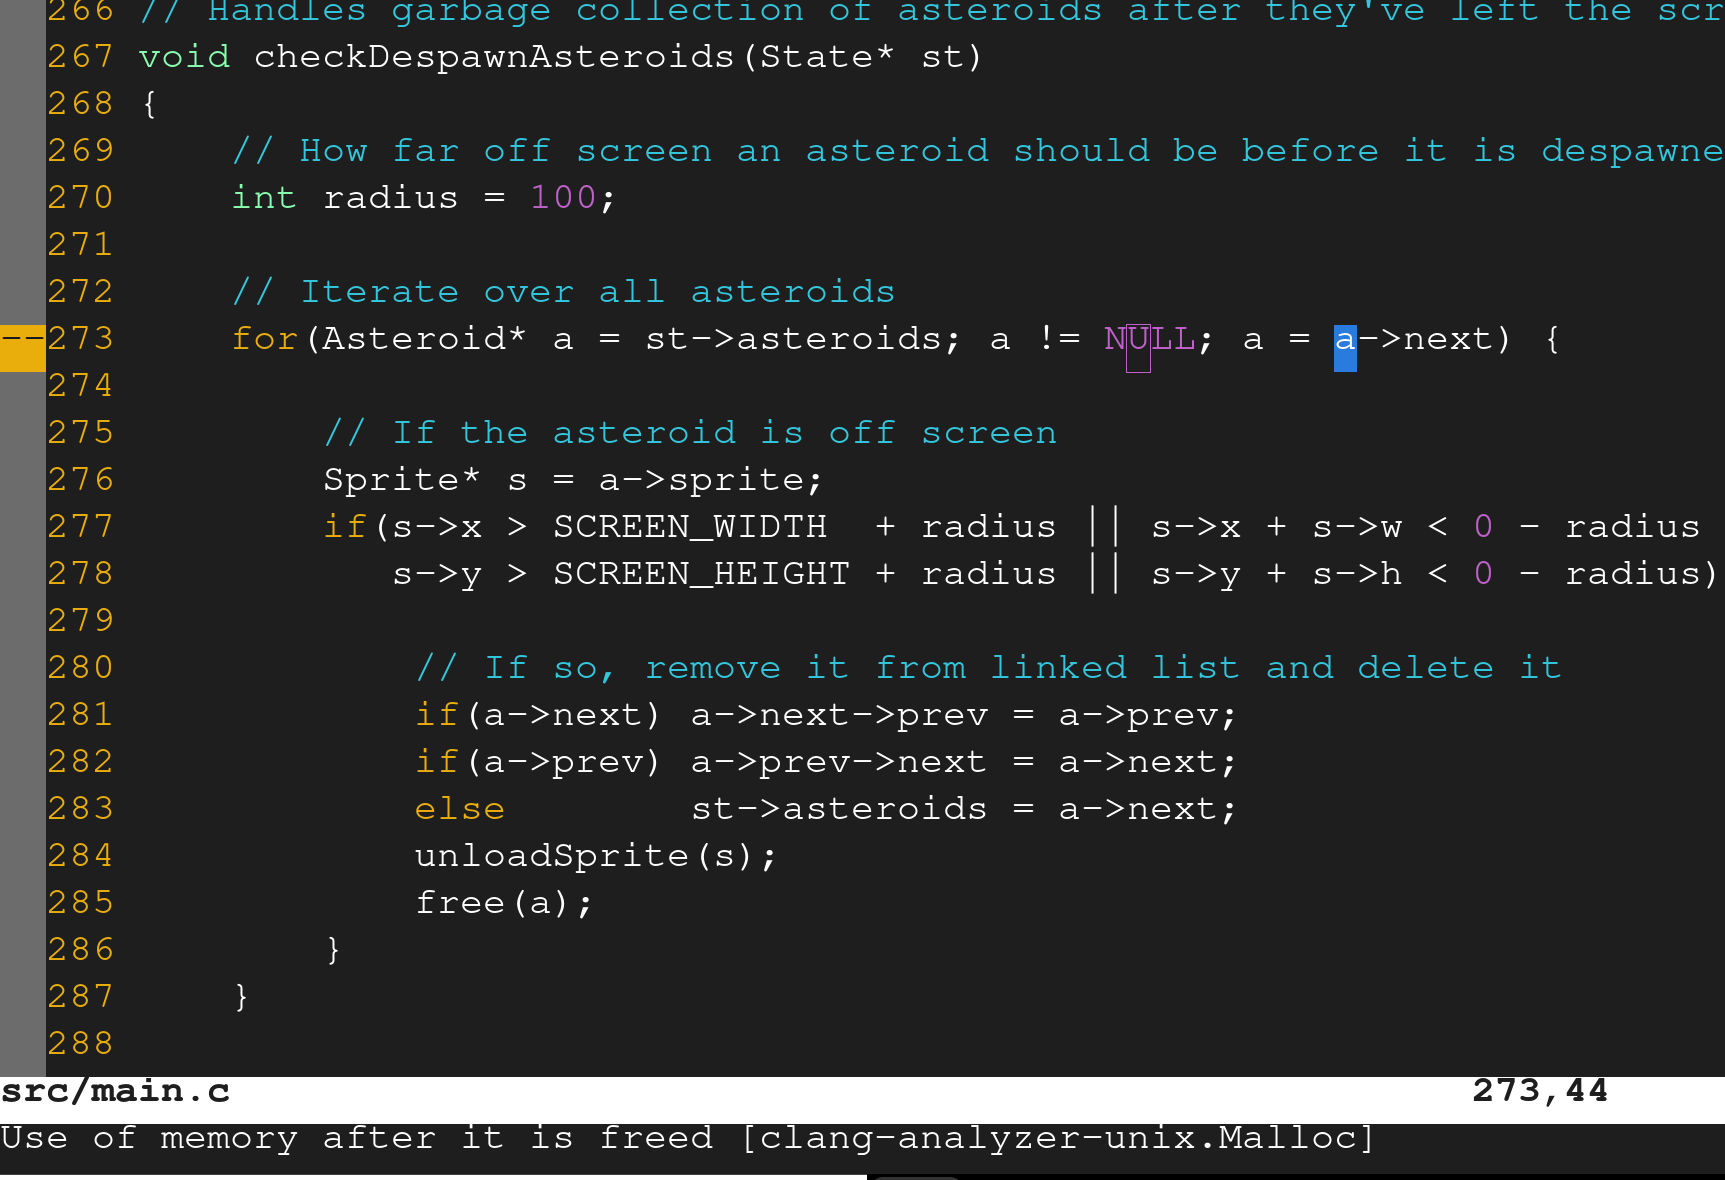
\includegraphics[width=\linewidth]{clang-tidy.png}
    \caption{Using \texttt{clang-tidy}}
    \label{fig:clang-tidy}
\end{figure}

\subsection{Using \cbmc}
\subsubsection{Creating interface API for \cbmc}
In order to use \cbmc, we were forced to de-couple the implementation of our game with its graphical implementation.
When we try to invoke \cbmc on the \texttt{SDL} library, even with the simplest code listing as below:
\begin{verbatim}
#include<SDL2/SDL.h>
int main(){}
\end{verbatim}
results in an error as shown in Figure~\ref{fig:cbmc-sdl}, even though the code runs properly.

\begin{figure}[!h]
    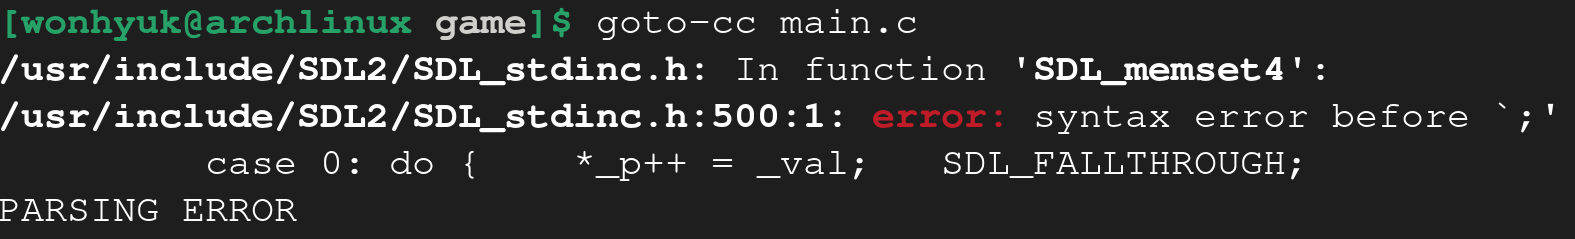
\includegraphics[width=\linewidth]{cbmc-sdl.png}
    \caption{Error with SDL2 and CBMC}
    \label{fig:cbmc-sdl}
\end{figure}

We decided to create a mock interface that has the same definitions of the library, without its implementations,
since we were not interested in checking the correctness of the \texttt{SDL} library.

\subsubsection{Writing good properties}
We found that writing properties was actually difficult -- creating the specification of the project was a major problem.


\subsubsection{Limited size checking of BMC}
As with all code, our codebase heavily relies on loops, and this exploded the size of our problem.
Even when we ran loops with depth $2$, they were heavily nested and took more than ten minutes to run.

Additionally, we wanted to check properties that are preserved across different functions calls (e.g. that the plane and the laser never collide), and so it was not always possible to instantiate environment assumptions for each function call.

\subsubsection{Debugging long error traces}
When we were able to find violations in our properties, we found that the counterexample traces that we found were very long.
For instance, for checking that our ship was in bounds, we obtained a counterexample trace (cf. Appendix ~\ref{appendix:trace}) that was $199$ transitions long.
This made debugging the property very difficult -- although perhaps a subtle error that we would not have been able to obtain without formal verification.

\section{Completed Project}
The completed game (Figure~\ref{fig:gameplay}) involves a plane and asteroids that move around according to the laws of physics (i.e. velocity and acceleration).

\begin{figure}[!h]
    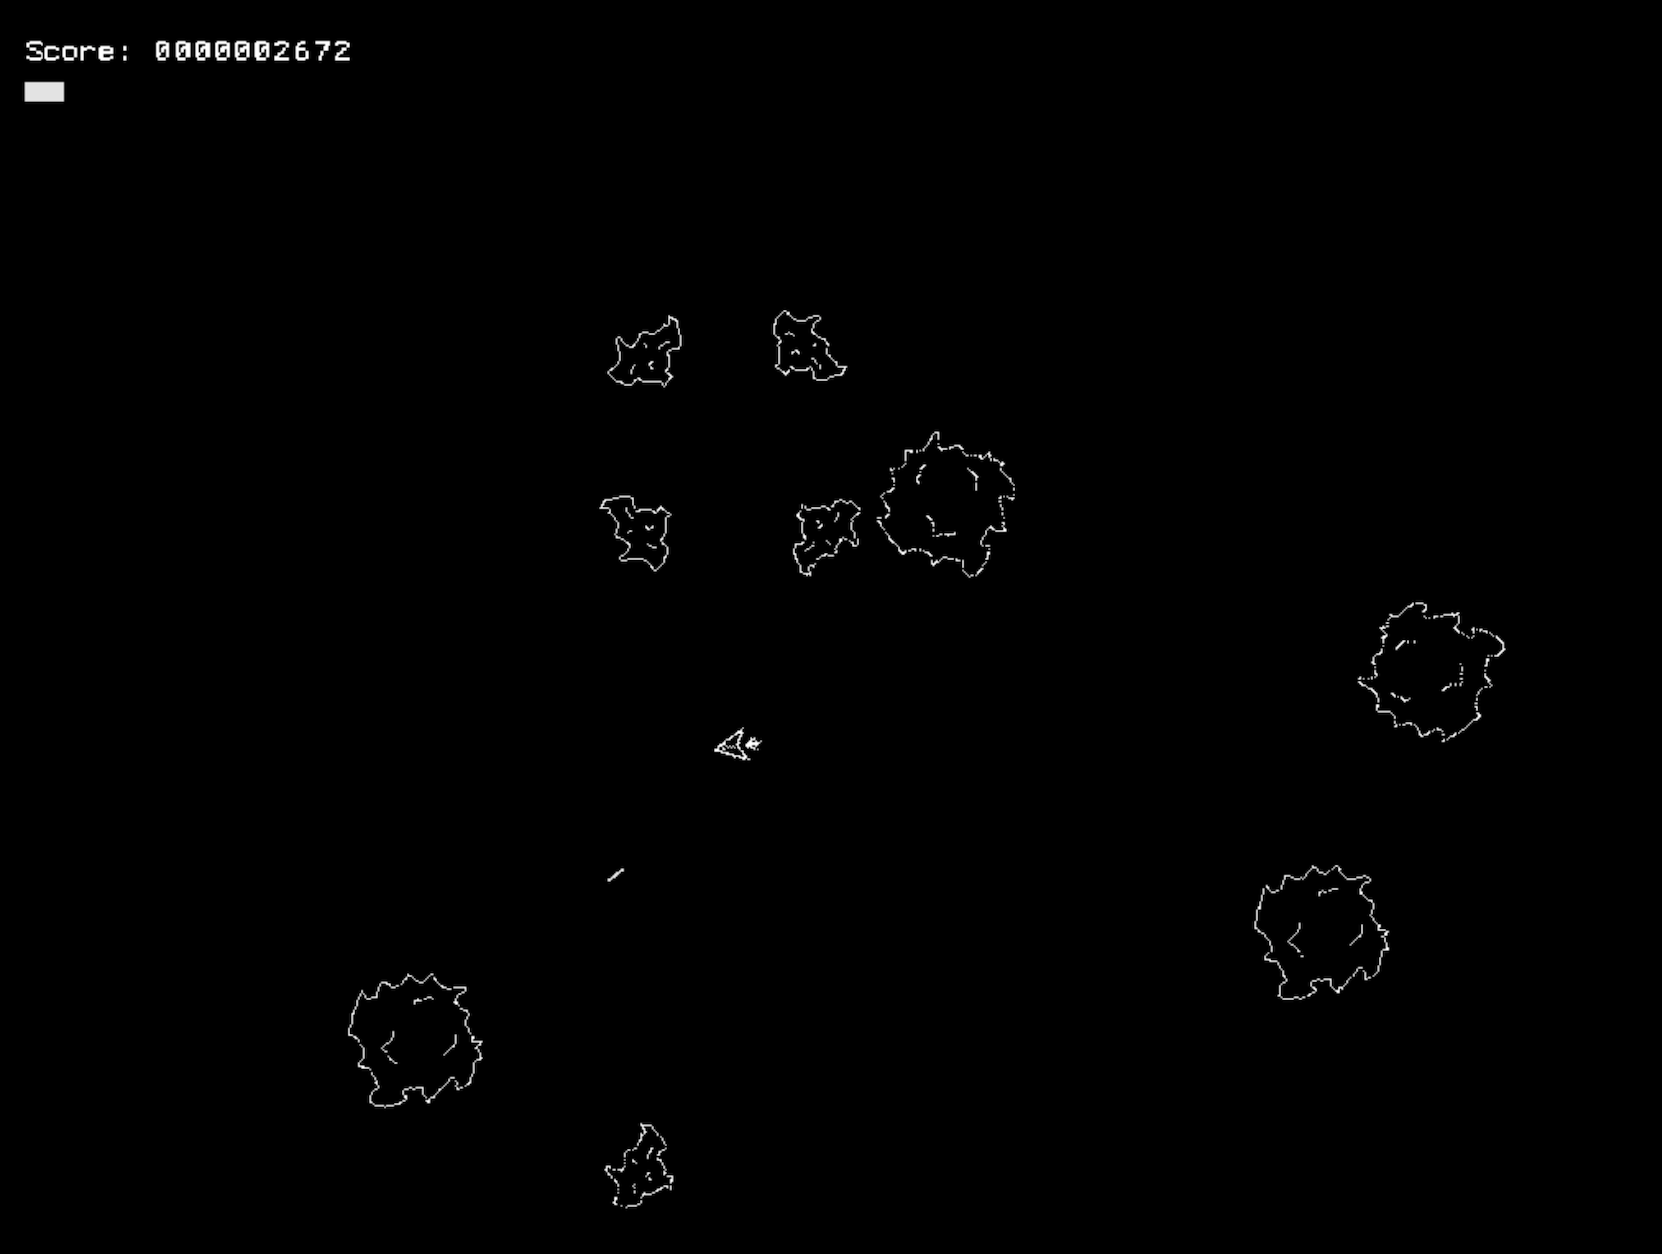
\includegraphics[width=\linewidth]{gameplay.png}
    \caption{Screenshot of \Name}
    \label{fig:gameplay}
\end{figure}

\section{Lessons Learned}

\bibliographystyle{IEEEtran}
\bibliography{proposal}

\appendix
\section{Counterexample Trace for Property Violation}
\label{appendix:trace}
\begin{verbatim}
src/main.c function moveShip
[moveShip.assertion.1] line 401 OOB: FAILURE

src/main.c function fireLaser
[fireLaser.assertion.1] line 508 Ship dx faster than laser!: SUCCESS
[fireLaser.assertion.2] line 510 Ship dy faster than laser!: SUCCESS

src/main.c function updateGame
[updateGame.precondition_instance.1] line 544 : SUCCESS

Trace for moveShip.assertion.1:

State 23 function __CPROVER__start thread 0
----------------------------------------------------
  INPUT argc: 1 (00000000 00000000 00000000 00000001)

State 27 file src/main.c function __CPROVER__start line 637 thread 0
----------------------------------------------------
  argc=1 (00000000 00000000 00000000 00000001)

State 28 file src/main.c function __CPROVER__start line 637 thread 0
----------------------------------------------------
  argv=argv' (00011000 00000000 00000000 00000000 00000000 00000000 00000000 00000000)

State 30 file src/main.c function main line 665 thread 0
----------------------------------------------------
  st={ .score=0l, .ship=((Sprite *)NULL), .laser_cooldown=0, .thrust=FALSE,
    .$pad4=0, .sprites=((SpriteList *)NULL) } ({ 00000000 00000000 00000000 00000000 00000000 00000000 00000000 00000000, 00000000 00000000 00000000 00000000 00000000 00000000 00000000 00000000, 00000000 00000000 00000000 00000000, 00000000, 00000000 00000000 00000000, 00000000 00000000 00000000 00000000 00000000 00000000 00000000 00000000 })

State 34 file src/main.c function main line 666 thread 0
----------------------------------------------------
  st=&st!0@1 (00011101 00000000 00000000 00000000 00000000 00000000 00000000 00000000)

State 35 file src/main.c function loadGame line 160 thread 0
----------------------------------------------------
  ship_w=0 (00000000 00000000 00000000 00000000)

State 36 file src/main.c function loadGame line 160 thread 0
----------------------------------------------------
  ship_w=20 (00000000 00000000 00000000 00010100)

State 37 file src/main.c function loadGame line 161 thread 0
----------------------------------------------------
  ship_h=0 (00000000 00000000 00000000 00000000)

State 38 file src/main.c function loadGame line 161 thread 0
----------------------------------------------------
  ship_h=20 (00000000 00000000 00000000 00010100)

State 39 file src/main.c function loadGame line 164 thread 0
----------------------------------------------------
  tm={ .tv_sec=0l, .tv_usec=1751545022280197l } ({ 00000000 00000000 00000000 00000000 00000000 00000000 00000000 00000000, 00000000 00000110 00111001 00000101 01011010 11011100 01110010 00000101 })

State 49 file src/main.c function loadGame line 169 thread 0
----------------------------------------------------
  a=1 (00000000 00000000 00000000 00000001)

State 56 file src/main.c function loadGame line 172 thread 0
----------------------------------------------------
  a=&'F' (00011110 00000000 00000000 00000000 00000000 00000000 00000000 00000000)

State 57 file src/main.c function loadGame line 172 thread 0
----------------------------------------------------
  b=20 (00000000 00000000 00000000 00010100)

State 58 file src/main.c function loadGame line 172 thread 0
----------------------------------------------------
  c=0 (00000000 00000000 00000000 00000000)

State 59 file src/main.c function loadGame line 172 thread 0
----------------------------------------------------
  d=1024 (00000000 00000000 00000100 00000000)

State 60 file src/main.c function loadGame line 172 thread 0
----------------------------------------------------
  e=768 (00000000 00000000 00000011 00000000)

State 61 file src/main.c function loadGame line 172 thread 0
----------------------------------------------------
  f=0 (00000000 00000000 00000000 00000000)

State 64 file src/main.c function loadGame line 172 thread 0
----------------------------------------------------
  window=((signed int *)NULL) + 1l (00000000 00000000 00000000 00000000 00000000 00000000 00000000 00000001)

State 68 file src/main.c function loadGame line 176 thread 0
----------------------------------------------------
  a=((signed int *)NULL) + 1l (00000000 00000000 00000000 00000000 00000000 00000000 00000000 00000001)

State 69 file src/main.c function loadGame line 176 thread 0
----------------------------------------------------
  b=-1 (11111111 11111111 11111111 11111111)

State 70 file src/main.c function loadGame line 176 thread 0
----------------------------------------------------
  c=2 (00000000 00000000 00000000 00000010)

State 73 file src/main.c function loadGame line 176 thread 0
----------------------------------------------------
  renderer=((signed int *)NULL) + 1l (00000000 00000000 00000000 00000000 00000000 00000000 00000000 00000001)

State 77 file src/main.c function loadGame line 180 thread 0
----------------------------------------------------
  a=((signed int *)NULL) + 1l (00000000 00000000 00000000 00000000 00000000 00000000 00000000 00000001)

State 78 file src/main.c function loadGame line 180 thread 0
----------------------------------------------------
  b=0 (00000000 00000000 00000000 00000000)

State 79 file src/main.c function loadGame line 180 thread 0
----------------------------------------------------
  c=0 (00000000 00000000 00000000 00000000)

State 80 file src/main.c function loadGame line 180 thread 0
----------------------------------------------------
  d=0 (00000000 00000000 00000000 00000000)

State 81 file src/main.c function loadGame line 180 thread 0
----------------------------------------------------
  e=255 (00000000 00000000 00000000 11111111)

State 89 file src/main.c function loadGame line 184 thread 0
----------------------------------------------------
  a=&'g' (00011111 00000000 00000000 00000000 00000000 00000000 00000000 00000000)

State 90 file src/main.c function loadGame line 184 thread 0
----------------------------------------------------
  b=24 (00000000 00000000 00000000 00011000)

State 93 file src/main.c function loadGame line 184 thread 0
----------------------------------------------------
  font=((signed int *)NULL) (00000000 00000000 00000000 00000000 00000000 00000000 00000000 00000000)

State 96 file src/main.c function loadGame line 187 thread 0
----------------------------------------------------
  a=44100 (00000000 00000000 10101100 01000100)

State 97 file src/main.c function loadGame line 187 thread 0
----------------------------------------------------
  b=6 (00000000 00000000 00000000 00000110)

State 98 file src/main.c function loadGame line 187 thread 0
----------------------------------------------------
  c=2 (00000000 00000000 00000000 00000010)

State 99 file src/main.c function loadGame line 187 thread 0
----------------------------------------------------
  d=2048 (00000000 00000000 00001000 00000000)

State 101 file src/main.c function loadGame line 190 thread 0
----------------------------------------------------
  track_select=0.0 (00000000 00000000 00000000 00000000 00000000 00000000 00000000 00000000)

State 111 file src/main.c function loadGame line 190 thread 0
----------------------------------------------------
  track_select=0.0 (00000000 00000000 00000000 00000000 00000000 00000000 00000000 00000000)

State 115 file src/main.c function loadGame line 191 thread 0
----------------------------------------------------
  a=&'a' (00100000 00000000 00000000 00000000 00000000 00000000 00000000 00000000)

State 118 file src/main.c function loadGame line 191 thread 0
----------------------------------------------------
  music=((signed int *)NULL) (00000000 00000000 00000000 00000000 00000000 00000000 00000000 00000000)

State 122 file src/main.c function loadGame line 193 thread 0
----------------------------------------------------
  a=100 (00000000 00000000 00000000 01100100)

State 126 file src/main.c function loadGame line 194 thread 0
----------------------------------------------------
  a=((signed int *)NULL) (00000000 00000000 00000000 00000000 00000000 00000000 00000000 00000000)

State 127 file src/main.c function loadGame line 194 thread 0
----------------------------------------------------
  b=-1 (11111111 11111111 11111111 11111111)

State 132 file src/main.c function loadGame line 197 thread 0
----------------------------------------------------
  malloc_size=16ul (00000000 00000000 00000000 00000000 00000000 00000000 00000000 00010000)

State 150 file src/main.c function loadGame line 197 thread 0
----------------------------------------------------
  sfx=dynamic_object1 (00100010 00000000 00000000 00000000 00000000 00000000 00000000 00000000)

State 153 file src/main.c function loadGame line 200 thread 0
----------------------------------------------------
  a=&'a' (00100011 00000000 00000000 00000000 00000000 00000000 00000000 00000000)

State 156 file src/main.c function loadGame line 200 thread 0
----------------------------------------------------
  dynamic_object1[0l]=((signed int *)NULL) (00000000 00000000 00000000 00000000 00000000 00000000 00000000 00000000)

State 159 file src/main.c function loadGame line 201 thread 0
----------------------------------------------------
  a=&'a' (00100100 00000000 00000000 00000000 00000000 00000000 00000000 00000000)

State 162 file src/main.c function loadGame line 201 thread 0
----------------------------------------------------
  dynamic_object1[1l]=((signed int *)NULL) (00000000 00000000 00000000 00000000 00000000 00000000 00000000 00000000)

State 163 file src/main.c function loadGame line 204 thread 0
----------------------------------------------------
  c_x=0.0 (00000000 00000000 00000000 00000000 00000000 00000000 00000000 00000000)

State 164 file src/main.c function loadGame line 204 thread 0
----------------------------------------------------
  c_x=502.0 (01000000 01111111 01100000 00000000 00000000 00000000 00000000 00000000)

State 165 file src/main.c function loadGame line 205 thread 0
----------------------------------------------------
  c_y=0.0 (00000000 00000000 00000000 00000000 00000000 00000000 00000000 00000000)

State 166 file src/main.c function loadGame line 205 thread 0
----------------------------------------------------
  c_y=374.0 (01000000 01110111 01100000 00000000 00000000 00000000 00000000 00000000)

State 169 file src/main.c function loadGame line 206 thread 0
----------------------------------------------------
  id=3 (00000000 00000000 00000000 00000011)

State 170 file src/main.c function loadGame line 206 thread 0
----------------------------------------------------
  w=20 (00000000 00000000 00000000 00010100)

State 171 file src/main.c function loadGame line 206 thread 0
----------------------------------------------------
  h=20 (00000000 00000000 00000000 00010100)

State 172 file src/main.c function loadGame line 206 thread 0
----------------------------------------------------
  x=502.0 (01000000 01111111 01100000 00000000 00000000 00000000 00000000 00000000)

State 173 file src/main.c function loadGame line 206 thread 0
----------------------------------------------------
  y=374.0 (01000000 01110111 01100000 00000000 00000000 00000000 00000000 00000000)

State 174 file src/main.c function loadGame line 206 thread 0
----------------------------------------------------
  path=&'g' (00100101 00000000 00000000 00000000 00000000 00000000 00000000 00000000)

State 175 file src/main.c function loadSprite line 46 thread 0
----------------------------------------------------
  s=((struct Sprite { signed int id; unsigned int $pad1; signed int *t; signed int w; signed int h; double x; double y; double theta; double dx; double dy; double omega; } *)NULL) (00000000 00000000 00000000 00000000 00000000 00000000 00000000 00000000)

State 179 file src/main.c function loadSprite line 46 thread 0
----------------------------------------------------
  malloc_size=72ul (00000000 00000000 00000000 00000000 00000000 00000000 00000000 01001000)

State 197 file src/main.c function loadSprite line 46 thread 0
----------------------------------------------------
  s=&dynamic_object2 (00100110 00000000 00000000 00000000 00000000 00000000 00000000 00000000)

State 198 file src/main.c function loadSprite line 47 thread 0
----------------------------------------------------
  dynamic_object2.id=3 (00000000 00000000 00000000 00000011)

State 201 file src/main.c function loadSprite line 48 thread 0
----------------------------------------------------
  path=&'g' (00100101 00000000 00000000 00000000 00000000 00000000 00000000 00000000)

State 202 file src/main.c function loadTexture line 28 thread 0
----------------------------------------------------
  newTexture=((signed int *)NULL) (00000000 00000000 00000000 00000000 00000000 00000000 00000000 00000000)

State 203 file src/main.c function loadTexture line 28 thread 0
----------------------------------------------------
  newTexture=((signed int *)NULL) (00000000 00000000 00000000 00000000 00000000 00000000 00000000 00000000)

State 204 file src/main.c function loadTexture line 29 thread 0
----------------------------------------------------
  loaded=((signed int *)NULL) (00000000 00000000 00000000 00000000 00000000 00000000 00000000 00000000)

State 207 file src/main.c function loadTexture line 29 thread 0
----------------------------------------------------
  a=&'g' (00100101 00000000 00000000 00000000 00000000 00000000 00000000 00000000)

State 210 file src/main.c function loadTexture line 29 thread 0
----------------------------------------------------
  loaded=((signed int *)NULL) (00000000 00000000 00000000 00000000 00000000 00000000 00000000 00000000)

State 213 file src/main.c function loadTexture line 32 thread 0
----------------------------------------------------
  a=((signed int *)NULL) + 1l (00000000 00000000 00000000 00000000 00000000 00000000 00000000 00000001)

State 214 file src/main.c function loadTexture line 32 thread 0
----------------------------------------------------
  b=((signed int *)NULL) (00000000 00000000 00000000 00000000 00000000 00000000 00000000 00000000)

State 217 file src/main.c function loadTexture line 32 thread 0
----------------------------------------------------
  newTexture=((signed int *)NULL) (00000000 00000000 00000000 00000000 00000000 00000000 00000000 00000000)

State 220 file src/main.c function loadTexture line 33 thread 0
----------------------------------------------------
  a=((signed int *)NULL) (00000000 00000000 00000000 00000000 00000000 00000000 00000000 00000000)

State 224 file src/main.c function loadSprite line 48 thread 0
----------------------------------------------------
  dynamic_object2.t=((signed int *)NULL) (00000000 00000000 00000000 00000000 00000000 00000000 00000000 00000000)

State 225 file src/main.c function loadSprite line 49 thread 0
----------------------------------------------------
  dynamic_object2.w=20 (00000000 00000000 00000000 00010100)

State 226 file src/main.c function loadSprite line 50 thread 0
----------------------------------------------------
  dynamic_object2.h=20 (00000000 00000000 00000000 00010100)

State 227 file src/main.c function loadSprite line 51 thread 0
----------------------------------------------------
  dynamic_object2.x=502.0 (01000000 01111111 01100000 00000000 00000000 00000000 00000000 00000000)

State 228 file src/main.c function loadSprite line 52 thread 0
----------------------------------------------------
  dynamic_object2.y=374.0 (01000000 01110111 01100000 00000000 00000000 00000000 00000000 00000000)

State 229 file src/main.c function loadSprite line 53 thread 0
----------------------------------------------------
  dynamic_object2.theta=1.570796 (00111111 11111001 00100001 11111011 01010100 01000100 00101101 00011000)

State 230 file src/main.c function loadSprite line 54 thread 0
----------------------------------------------------
  dynamic_object2.dx=0.0 (00000000 00000000 00000000 00000000 00000000 00000000 00000000 00000000)

State 231 file src/main.c function loadSprite line 55 thread 0
----------------------------------------------------
  dynamic_object2.dy=0.0 (00000000 00000000 00000000 00000000 00000000 00000000 00000000 00000000)

State 232 file src/main.c function loadSprite line 56 thread 0
----------------------------------------------------
  dynamic_object2.omega=0.0 (00000000 00000000 00000000 00000000 00000000 00000000 00000000 00000000)

State 235 file src/main.c function loadGame line 206 thread 0
----------------------------------------------------
  st.ship=&dynamic_object2 (00100110 00000000 00000000 00000000 00000000 00000000 00000000 00000000)

State 236 file src/main.c function loadGame line 207 thread 0
----------------------------------------------------
  st.score=0l (00000000 00000000 00000000 00000000 00000000 00000000 00000000 00000000)

State 237 file src/main.c function loadGame line 208 thread 0
----------------------------------------------------
  st.laser_cooldown=0 (00000000 00000000 00000000 00000000)

State 238 file src/main.c function loadGame line 209 thread 0
----------------------------------------------------
  st.thrust=FALSE (00000000)

State 239 file src/main.c function loadGame line 212 thread 0
----------------------------------------------------
  st.sprites=((SpriteList *)NULL) (00000000 00000000 00000000 00000000 00000000 00000000 00000000 00000000)

State 242 file src/main.c function loadGame line 213 thread 0
----------------------------------------------------
  st=&st!0@1 (00011101 00000000 00000000 00000000 00000000 00000000 00000000 00000000)

State 247 file src/main.c function ensureAsteroids line 149 thread 0
----------------------------------------------------
  st=&st!0@1 (00011101 00000000 00000000 00000000 00000000 00000000 00000000 00000000)

State 248 file src/main.c function spawnAsteroid line 76 thread 0
----------------------------------------------------
  a_w=0 (00000000 00000000 00000000 00000000)

State 249 file src/main.c function spawnAsteroid line 76 thread 0
----------------------------------------------------
  a_w=84 (00000000 00000000 00000000 01010100)

State 250 file src/main.c function spawnAsteroid line 77 thread 0
----------------------------------------------------
  a_h=0 (00000000 00000000 00000000 00000000)

State 251 file src/main.c function spawnAsteroid line 77 thread 0
----------------------------------------------------
  a_h=83 (00000000 00000000 00000000 01010011)

State 252 file src/main.c function spawnAsteroid line 81 thread 0
----------------------------------------------------
  ratio=0.0 (00000000 00000000 00000000 00000000 00000000 00000000 00000000 00000000)

State 253 file src/main.c function spawnAsteroid line 81 thread 0
----------------------------------------------------
  ratio=1.333333 (00111111 11110101 01010101 01010101 01010101 01010101 01010101 01010101)

State 254 file src/main.c function spawnAsteroid line 82 thread 0
----------------------------------------------------
  weighted_chance=0.0 (00000000 00000000 00000000 00000000 00000000 00000000 00000000 00000000)

State 255 file src/main.c function spawnAsteroid line 82 thread 0
----------------------------------------------------
  weighted_chance=0.666667 (00111111 11100101 01010101 01010101 01010101 01010101 01010101 01010101)

State 256 file src/main.c function spawnAsteroid line 85 thread 0
----------------------------------------------------
  x=0.0 (00000000 00000000 00000000 00000000 00000000 00000000 00000000 00000000)

State 257 file src/main.c function spawnAsteroid line 85 thread 0
----------------------------------------------------
  x=0.0 (00000000 00000000 00000000 00000000 00000000 00000000 00000000 00000000)

State 258 file src/main.c function spawnAsteroid line 86 thread 0
----------------------------------------------------
  y=0.0 (00000000 00000000 00000000 00000000 00000000 00000000 00000000 00000000)

State 259 file src/main.c function spawnAsteroid line 86 thread 0
----------------------------------------------------
  y=0.0 (00000000 00000000 00000000 00000000 00000000 00000000 00000000 00000000)

State 260 file src/main.c function spawnAsteroid line 87 thread 0
----------------------------------------------------
  dx=0.0 (00000000 00000000 00000000 00000000 00000000 00000000 00000000 00000000)

State 274 file src/main.c function spawnAsteroid line 87 thread 0
----------------------------------------------------
  a=1.343875 (00111111 11110101 10000000 10000010 11100101 10101011 00000001 00000110)

State 275 file src/main.c function spawnAsteroid line 87 thread 0
----------------------------------------------------
  b=3.0 (01000000 00001000 00000000 00000000 00000000 00000000 00000000 00000000)

State 280 file src/main.c function spawnAsteroid line 87 thread 0
----------------------------------------------------
  dx=1.343875 (00111111 11110101 10000000 10000010 11100101 10101011 00000001 00000110)

State 281 file src/main.c function spawnAsteroid line 88 thread 0
----------------------------------------------------
  dy=0.0 (00000000 00000000 00000000 00000000 00000000 00000000 00000000 00000000)

State 295 file src/main.c function spawnAsteroid line 88 thread 0
----------------------------------------------------
  a=2.561137e-9 (00111110 00100110 00000000 00000000 00000000 00000000 00000000 00000000)

State 296 file src/main.c function spawnAsteroid line 88 thread 0
----------------------------------------------------
  b=3.0 (01000000 00001000 00000000 00000000 00000000 00000000 00000000 00000000)

State 301 file src/main.c function spawnAsteroid line 88 thread 0
----------------------------------------------------
  dy=2.561137e-9 (00111110 00100110 00000000 00000000 00000000 00000000 00000000 00000000)

State 302 file src/main.c function spawnAsteroid line 91 thread 0
----------------------------------------------------
  where=0.0 (00000000 00000000 00000000 00000000 00000000 00000000 00000000 00000000)

State 312 file src/main.c function spawnAsteroid line 91 thread 0
----------------------------------------------------
  where=0.63135 (00111111 11100100 00110100 00000100 11111010 00101000 01101000 00001010)

State 326 file src/main.c function spawnAsteroid line 100 thread 0
----------------------------------------------------
  x=-708.486346 (11000000 10000110 00100011 11100100 00001001 01110011 01000111 11001000)

State 327 file src/main.c function spawnAsteroid line 101 thread 0
----------------------------------------------------
  y=768.0 (01000000 10001000 00000000 00000000 00000000 00000000 00000000 00000000)

State 328 file src/main.c function spawnAsteroid line 102 thread 0
----------------------------------------------------
  dx=0.671937 (00111111 11100101 10000000 10000010 11100101 10101011 00000001 00000110)

State 329 file src/main.c function spawnAsteroid line 103 thread 0
----------------------------------------------------
  dy=-2.561137e-9 (10111110 00100110 00000000 00000000 00000000 00000000 00000000 00000000)

State 331 file src/main.c function spawnAsteroid line 122 thread 0
----------------------------------------------------
  a=((struct Sprite { signed int id; unsigned int $pad1; signed int *t; signed int w; signed int h; double x; double y; double theta; double dx; double dy; double omega; } *)NULL) (00000000 00000000 00000000 00000000 00000000 00000000 00000000 00000000)

State 334 file src/main.c function spawnAsteroid line 122 thread 0
----------------------------------------------------
  id=0 (00000000 00000000 00000000 00000000)

State 335 file src/main.c function spawnAsteroid line 122 thread 0
----------------------------------------------------
  w=84 (00000000 00000000 00000000 01010100)

State 336 file src/main.c function spawnAsteroid line 122 thread 0
----------------------------------------------------
  h=83 (00000000 00000000 00000000 01010011)

State 337 file src/main.c function spawnAsteroid line 122 thread 0
----------------------------------------------------
  x=-708.486346 (11000000 10000110 00100011 11100100 00001001 01110011 01000111 11001000)

State 338 file src/main.c function spawnAsteroid line 122 thread 0
----------------------------------------------------
  y=768.0 (01000000 10001000 00000000 00000000 00000000 00000000 00000000 00000000)

State 339 file src/main.c function spawnAsteroid line 122 thread 0
----------------------------------------------------
  path=&'g' (00100111 00000000 00000000 00000000 00000000 00000000 00000000 00000000)

State 340 file src/main.c function loadSprite line 46 thread 0
----------------------------------------------------
  s=((struct Sprite { signed int id; unsigned int $pad1; signed int *t; signed int w; signed int h; double x; double y; double theta; double dx; double dy; double omega; } *)NULL) (00000000 00000000 00000000 00000000 00000000 00000000 00000000 00000000)

State 344 file src/main.c function loadSprite line 46 thread 0
----------------------------------------------------
  malloc_size=72ul (00000000 00000000 00000000 00000000 00000000 00000000 00000000 01001000)

State 362 file src/main.c function loadSprite line 46 thread 0
----------------------------------------------------
  s=&dynamic_object3 (00010000 00000000 00000000 00000000 00000000 00000000 00000000 00000000)

State 363 file src/main.c function loadSprite line 47 thread 0
----------------------------------------------------
  dynamic_object3.id=0 (00000000 00000000 00000000 00000000)

State 366 file src/main.c function loadSprite line 48 thread 0
----------------------------------------------------
  path=&'g' (00100111 00000000 00000000 00000000 00000000 00000000 00000000 00000000)

State 367 file src/main.c function loadTexture line 28 thread 0
----------------------------------------------------
  newTexture=((signed int *)NULL) (00000000 00000000 00000000 00000000 00000000 00000000 00000000 00000000)

State 368 file src/main.c function loadTexture line 28 thread 0
----------------------------------------------------
  newTexture=((signed int *)NULL) (00000000 00000000 00000000 00000000 00000000 00000000 00000000 00000000)

State 369 file src/main.c function loadTexture line 29 thread 0
----------------------------------------------------
  loaded=((signed int *)NULL) (00000000 00000000 00000000 00000000 00000000 00000000 00000000 00000000)

State 372 file src/main.c function loadTexture line 29 thread 0
----------------------------------------------------
  a=&'g' (00100111 00000000 00000000 00000000 00000000 00000000 00000000 00000000)

State 375 file src/main.c function loadTexture line 29 thread 0
----------------------------------------------------
  loaded=((signed int *)NULL) (00000000 00000000 00000000 00000000 00000000 00000000 00000000 00000000)

State 378 file src/main.c function loadTexture line 32 thread 0
----------------------------------------------------
  a=((signed int *)NULL) + 1l (00000000 00000000 00000000 00000000 00000000 00000000 00000000 00000001)

State 379 file src/main.c function loadTexture line 32 thread 0
----------------------------------------------------
  b=((signed int *)NULL) (00000000 00000000 00000000 00000000 00000000 00000000 00000000 00000000)

State 382 file src/main.c function loadTexture line 32 thread 0
----------------------------------------------------
  newTexture=((signed int *)NULL) (00000000 00000000 00000000 00000000 00000000 00000000 00000000 00000000)

State 385 file src/main.c function loadTexture line 33 thread 0
----------------------------------------------------
  a=((signed int *)NULL) (00000000 00000000 00000000 00000000 00000000 00000000 00000000 00000000)

State 389 file src/main.c function loadSprite line 48 thread 0
----------------------------------------------------
  dynamic_object3.t=((signed int *)NULL) (00000000 00000000 00000000 00000000 00000000 00000000 00000000 00000000)

State 390 file src/main.c function loadSprite line 49 thread 0
----------------------------------------------------
  dynamic_object3.w=84 (00000000 00000000 00000000 01010100)

State 391 file src/main.c function loadSprite line 50 thread 0
----------------------------------------------------
  dynamic_object3.h=83 (00000000 00000000 00000000 01010011)

State 392 file src/main.c function loadSprite line 51 thread 0
----------------------------------------------------
  dynamic_object3.x=-708.486346 (11000000 10000110 00100011 11100100 00001001 01110011 01000111 11001000)

State 393 file src/main.c function loadSprite line 52 thread 0
----------------------------------------------------
  dynamic_object3.y=768.0 (01000000 10001000 00000000 00000000 00000000 00000000 00000000 00000000)

State 394 file src/main.c function loadSprite line 53 thread 0
----------------------------------------------------
  dynamic_object3.theta=1.570796 (00111111 11111001 00100001 11111011 01010100 01000100 00101101 00011000)

State 395 file src/main.c function loadSprite line 54 thread 0
----------------------------------------------------
  dynamic_object3.dx=0.0 (00000000 00000000 00000000 00000000 00000000 00000000 00000000 00000000)

State 396 file src/main.c function loadSprite line 55 thread 0
----------------------------------------------------
  dynamic_object3.dy=0.0 (00000000 00000000 00000000 00000000 00000000 00000000 00000000 00000000)

State 397 file src/main.c function loadSprite line 56 thread 0
----------------------------------------------------
  dynamic_object3.omega=0.0 (00000000 00000000 00000000 00000000 00000000 00000000 00000000 00000000)

State 400 file src/main.c function spawnAsteroid line 122 thread 0
----------------------------------------------------
  a=&dynamic_object3 (00010000 00000000 00000000 00000000 00000000 00000000 00000000 00000000)

State 401 file src/main.c function spawnAsteroid line 123 thread 0
----------------------------------------------------
  dynamic_object3.dx=0.671937 (00111111 11100101 10000000 10000010 11100101 10101011 00000001 00000110)

State 402 file src/main.c function spawnAsteroid line 124 thread 0
----------------------------------------------------
  dynamic_object3.dy=-2.561137e-9 (10111110 00100110 00000000 00000000 00000000 00000000 00000000 00000000)

State 414 file src/main.c function spawnAsteroid line 125 thread 0
----------------------------------------------------
  dynamic_object3.omega=-0.0 (10000000 00000000 00000000 00000000 00000000 00000000 00000000 00000000)

State 420 file src/main.c function ensureAsteroids line 149 thread 0
----------------------------------------------------
  st=&st!0@1 (00011101 00000000 00000000 00000000 00000000 00000000 00000000 00000000)

State 421 file src/main.c function ensureAsteroids line 149 thread 0
----------------------------------------------------
  s=&dynamic_object3 (00010000 00000000 00000000 00000000 00000000 00000000 00000000 00000000)

State 422 file src/main.c function addSprite line 63 thread 0
----------------------------------------------------
  head=((struct SpriteList { SpriteList *prev; SpriteList *next; Sprite *sprite; } *)NULL) (00000000 00000000 00000000 00000000 00000000 00000000 00000000 00000000)

State 426 file src/main.c function addSprite line 63 thread 0
----------------------------------------------------
  malloc_size=24ul (00000000 00000000 00000000 00000000 00000000 00000000 00000000 00011000)

State 444 file src/main.c function addSprite line 63 thread 0
----------------------------------------------------
  head=&dynamic_object4 (00000011 00000000 00000000 00000000 00000000 00000000 00000000 00000000)

State 445 file src/main.c function addSprite line 64 thread 0
----------------------------------------------------
  dynamic_object4.prev=((SpriteList *)NULL) (00000000 00000000 00000000 00000000 00000000 00000000 00000000 00000000)

State 446 file src/main.c function addSprite line 65 thread 0
----------------------------------------------------
  dynamic_object4.next=((SpriteList *)NULL) (00000000 00000000 00000000 00000000 00000000 00000000 00000000 00000000)

State 447 file src/main.c function addSprite line 66 thread 0
----------------------------------------------------
  dynamic_object4.sprite=&dynamic_object3 (00010000 00000000 00000000 00000000 00000000 00000000 00000000 00000000)

State 449 file src/main.c function addSprite line 68 thread 0
----------------------------------------------------
  st.sprites=&dynamic_object4 (00000011 00000000 00000000 00000000 00000000 00000000 00000000 00000000)

State 457 file src/main.c function main line 673 thread 0
----------------------------------------------------
  quit=FALSE (00000000)

State 458 file src/main.c function main line 673 thread 0
----------------------------------------------------
  quit=FALSE (00000000)

State 460 file src/main.c function main line 677 thread 0
----------------------------------------------------
  start_time=0 (00000000 00000000 00000000 00000000)

State 465 file src/main.c function main line 677 thread 0
----------------------------------------------------
  start_time=0 (00000000 00000000 00000000 00000000)

State 466 file src/main.c function main line 680 thread 0
----------------------------------------------------
  e={ .type=0, .key={ .keysym={ .sym=0 } } } ({ 00000000 00000000 00000000 00000000, { { 00000000 00000000 00000000 00000000 } } })

State 470 file src/main.c function main line 681 thread 0
----------------------------------------------------
  a=&e!0@1 (00101000 00000000 00000000 00000000 00000000 00000000 00000000 00000000)

State 471 file src/../headers/mockSDL.h function SDL_PollEvent line 52 thread 0
----------------------------------------------------
  e.type=100 (00000000 00000000 00000000 01100100)

State 476 file src/main.c function main line 685 thread 0
----------------------------------------------------
  keys=((signed int *)NULL) (00000000 00000000 00000000 00000000 00000000 00000000 00000000 00000000)

State 479 file src/main.c function main line 685 thread 0
----------------------------------------------------
  a=NULL (00000000 00000000 00000000 00000000 00000000 00000000 00000000 00000000)

State 482 file src/main.c function main line 685 thread 0
----------------------------------------------------
  keys=spoofKeystate (00101001 00000000 00000000 00000000 00000000 00000000 00000000 00000000)

State 486 file src/main.c function main line 686 thread 0
----------------------------------------------------
  st=&st!0@1 (00011101 00000000 00000000 00000000 00000000 00000000 00000000 00000000)

State 487 file src/main.c function main line 686 thread 0
----------------------------------------------------
  keys=spoofKeystate (00101001 00000000 00000000 00000000 00000000 00000000 00000000 00000000)

State 490 file src/main.c function updateGame line 528 thread 0
----------------------------------------------------
  st=&st!0@1 (00011101 00000000 00000000 00000000 00000000 00000000 00000000 00000000)

State 491 file src/main.c function updateGame line 528 thread 0
----------------------------------------------------
  keys=spoofKeystate (00101001 00000000 00000000 00000000 00000000 00000000 00000000 00000000)

State 492 file src/main.c function moveShip line 358 thread 0
----------------------------------------------------
  s=((struct Sprite { signed int id; unsigned int $pad1; signed int *t; signed int w; signed int h; double x; double y; double theta; double dx; double dy; double omega; } *)NULL) (00000000 00000000 00000000 00000000 00000000 00000000 00000000 00000000)

State 493 file src/main.c function moveShip line 358 thread 0
----------------------------------------------------
  s=&dynamic_object2 (00100110 00000000 00000000 00000000 00000000 00000000 00000000 00000000)

State 494 file src/main.c function moveShip line 361 thread 0
----------------------------------------------------
  thrust=0.0 (00000000 00000000 00000000 00000000 00000000 00000000 00000000 00000000)

State 495 file src/main.c function moveShip line 361 thread 0
----------------------------------------------------
  thrust=0.08 (00111111 10110100 01111010 11100001 01000111 10101110 00010100 01111011)

State 496 file src/main.c function moveShip line 362 thread 0
----------------------------------------------------
  thrust_damp=0.0 (00000000 00000000 00000000 00000000 00000000 00000000 00000000 00000000)

State 497 file src/main.c function moveShip line 362 thread 0
----------------------------------------------------
  thrust_damp=0.99 (00111111 11101111 10101110 00010100 01111010 11100001 01000111 10101110)

State 498 file src/main.c function moveShip line 363 thread 0
----------------------------------------------------
  torque=0.0 (00000000 00000000 00000000 00000000 00000000 00000000 00000000 00000000)

State 499 file src/main.c function moveShip line 363 thread 0
----------------------------------------------------
  torque=0.004 (00111111 01110000 01100010 01001101 11010010 11110001 10101001 11111100)

State 500 file src/main.c function moveShip line 364 thread 0
----------------------------------------------------
  torque_damp=0.0 (00000000 00000000 00000000 00000000 00000000 00000000 00000000 00000000)

State 501 file src/main.c function moveShip line 364 thread 0
----------------------------------------------------
  torque_damp=0.95 (00111111 11101110 01100110 01100110 01100110 01100110 01100110 01100110)

State 502 file src/main.c function moveShip line 367 thread 0
----------------------------------------------------
  dynamic_object2.dx=0.0 (00000000 00000000 00000000 00000000 00000000 00000000 00000000 00000000)

State 503 file src/main.c function moveShip line 368 thread 0
----------------------------------------------------
  dynamic_object2.dy=0.0 (00000000 00000000 00000000 00000000 00000000 00000000 00000000 00000000)

State 504 file src/main.c function moveShip line 369 thread 0
----------------------------------------------------
  dynamic_object2.omega=0.0 (00000000 00000000 00000000 00000000 00000000 00000000 00000000 00000000)

State 506 file src/main.c function moveShip line 373 thread 0
----------------------------------------------------
  st.thrust=TRUE (00000001)

State 510 file src/main.c function moveShip line 374 thread 0
----------------------------------------------------
  x=1.570796 (00111111 11111001 00100001 11111011 01010100 01000100 00101101 00011000)

State 511 file <builtin-library-cos> function cos line 7 thread 0
----------------------------------------------------
  ret=0.0 (00000000 00000000 00000000 00000000 00000000 00000000 00000000 00000000)

State 512 file <builtin-library-cos> function cos line 7 thread 0
----------------------------------------------------
  ret=2.820079e-12 (00111101 10001000 11001110 01000000 11110110 00010011 00011101 11111010)

State 520 file src/main.c function moveShip line 374 thread 0
----------------------------------------------------
  dynamic_object2.dx=2.256063e-13 (00111101 01001111 11000000 01010011 00100110 01111110 11011110 10110001)

State 524 file src/main.c function moveShip line 375 thread 0
----------------------------------------------------
  x=1.570796 (00111111 11111001 00100001 11111011 01010100 01000100 00101101 00011000)

State 525 file <builtin-library-sin> function sin line 7 thread 0
----------------------------------------------------
  ret=0.0 (00000000 00000000 00000000 00000000 00000000 00000000 00000000 00000000)

State 526 file <builtin-library-sin> function sin line 7 thread 0
----------------------------------------------------
  ret=-5.311244e-71 (10110001 01010111 01110101 11011100 00001101 01000100 00100011 11001011)

State 534 file src/main.c function moveShip line 375 thread 0
----------------------------------------------------
  dynamic_object2.dy=4.248995e-72 (00110001 00011110 00000111 10000000 00010000 11111011 00001111 00011000)

State 538 file src/main.c function moveShip line 388 thread 0
----------------------------------------------------
  dynamic_object2.x=502.0 (01000000 01111111 01100000 00000000 00000000 00000000 00000000 00000100)

State 539 file src/main.c function moveShip line 389 thread 0
----------------------------------------------------
  dynamic_object2.y=374.0 (01000000 01110111 01100000 00000000 00000000 00000000 00000000 00000000)

State 540 file src/main.c function moveShip line 390 thread 0
----------------------------------------------------
  dynamic_object2.theta=1.570796 (00111111 11111001 00100001 11111011 01010100 01000100 00101101 00011000)

State 545 file src/main.c function moveShip line 399 thread 0
----------------------------------------------------
  xOutOfBounds=FALSE (00000000)

State 550 file src/main.c function moveShip line 399 thread 0
----------------------------------------------------
  xOutOfBounds=TRUE (00000001)

State 551 file src/main.c function moveShip line 400 thread 0
----------------------------------------------------
  yOutOfBounds=FALSE (00000000)

State 556 file src/main.c function moveShip line 400 thread 0
----------------------------------------------------
  yOutOfBounds=TRUE (00000001)

Violated property:
  file src/main.c function moveShip line 401 thread 0
  OOB
  !(xOutOfBounds != FALSE || yOutOfBounds != FALSE)

** 1 of 22 failed (2 iterations)
VERIFICATION FAILED
  
\end{verbatim}

\end{document}
